% ----------------------------------------------------------------------------
\chapter{Multiprocesszoros program}
% ----------------------------------------------------------------------------
\section{A szimulátor dekomponálása a párhuzamos feladatokra}

\section{A szimulátor bemutatása} 
	 A prototípus algoritmus fejlesztése MATLAB környezetben történt, ami a későbbi referenciaként szolgál.
	 Alap MATLAB utasításokat használva több órát vesz igénybe a szimuláció futtatása.
	 A MATLAB Parallel Toolbox-nak segítségével a szimulációt lehetséges párhuzamosan több processzormagon futtatni.
	 Ezzel párszoros sebesség növekezés érhető el a MATLAB magas nyelvű programnyelve végett.
	 A következőkben magát az algoritmust és az OpenCL keretrendszerben történő implementációját mutatom be.
	 Majd az eredmények bemutatása után összevetésre kerül a MATLAB referencia, a MATLAB Parallel Toolbox segítséggel,
	 az OpenCL processzoron és az OpenCL GPU-n való futási ideje.
	
\section{A lépések részletezése} 
\subsection{Interpoláció}
	A korábban elmondottak alapján a felületet további virtuális pontokkal egészítjük ki.
	Az virtuális mérési pontokat a legegyszerűbben bilineáris interpolációval (síklapos közelítéssel) becsülhetjük.
	\begin{changebar}
	A szimulátorban egy általánosabb módszert alkalmazunk, ami egy 2D-s mozgó átlagoló szűrővel való simítás.
	A szűrővel aluláteresztést tudunk elérni, ami a minta magasságának mintavételezése utáni rekonstrukcióját jelenti.
	\end{changebar}
	Egy ilyen interpoláció eredményét láthatjuk a \ref{fig:33pont}. ábrán.
	
	\begin{figure}[!h]
		\centering
		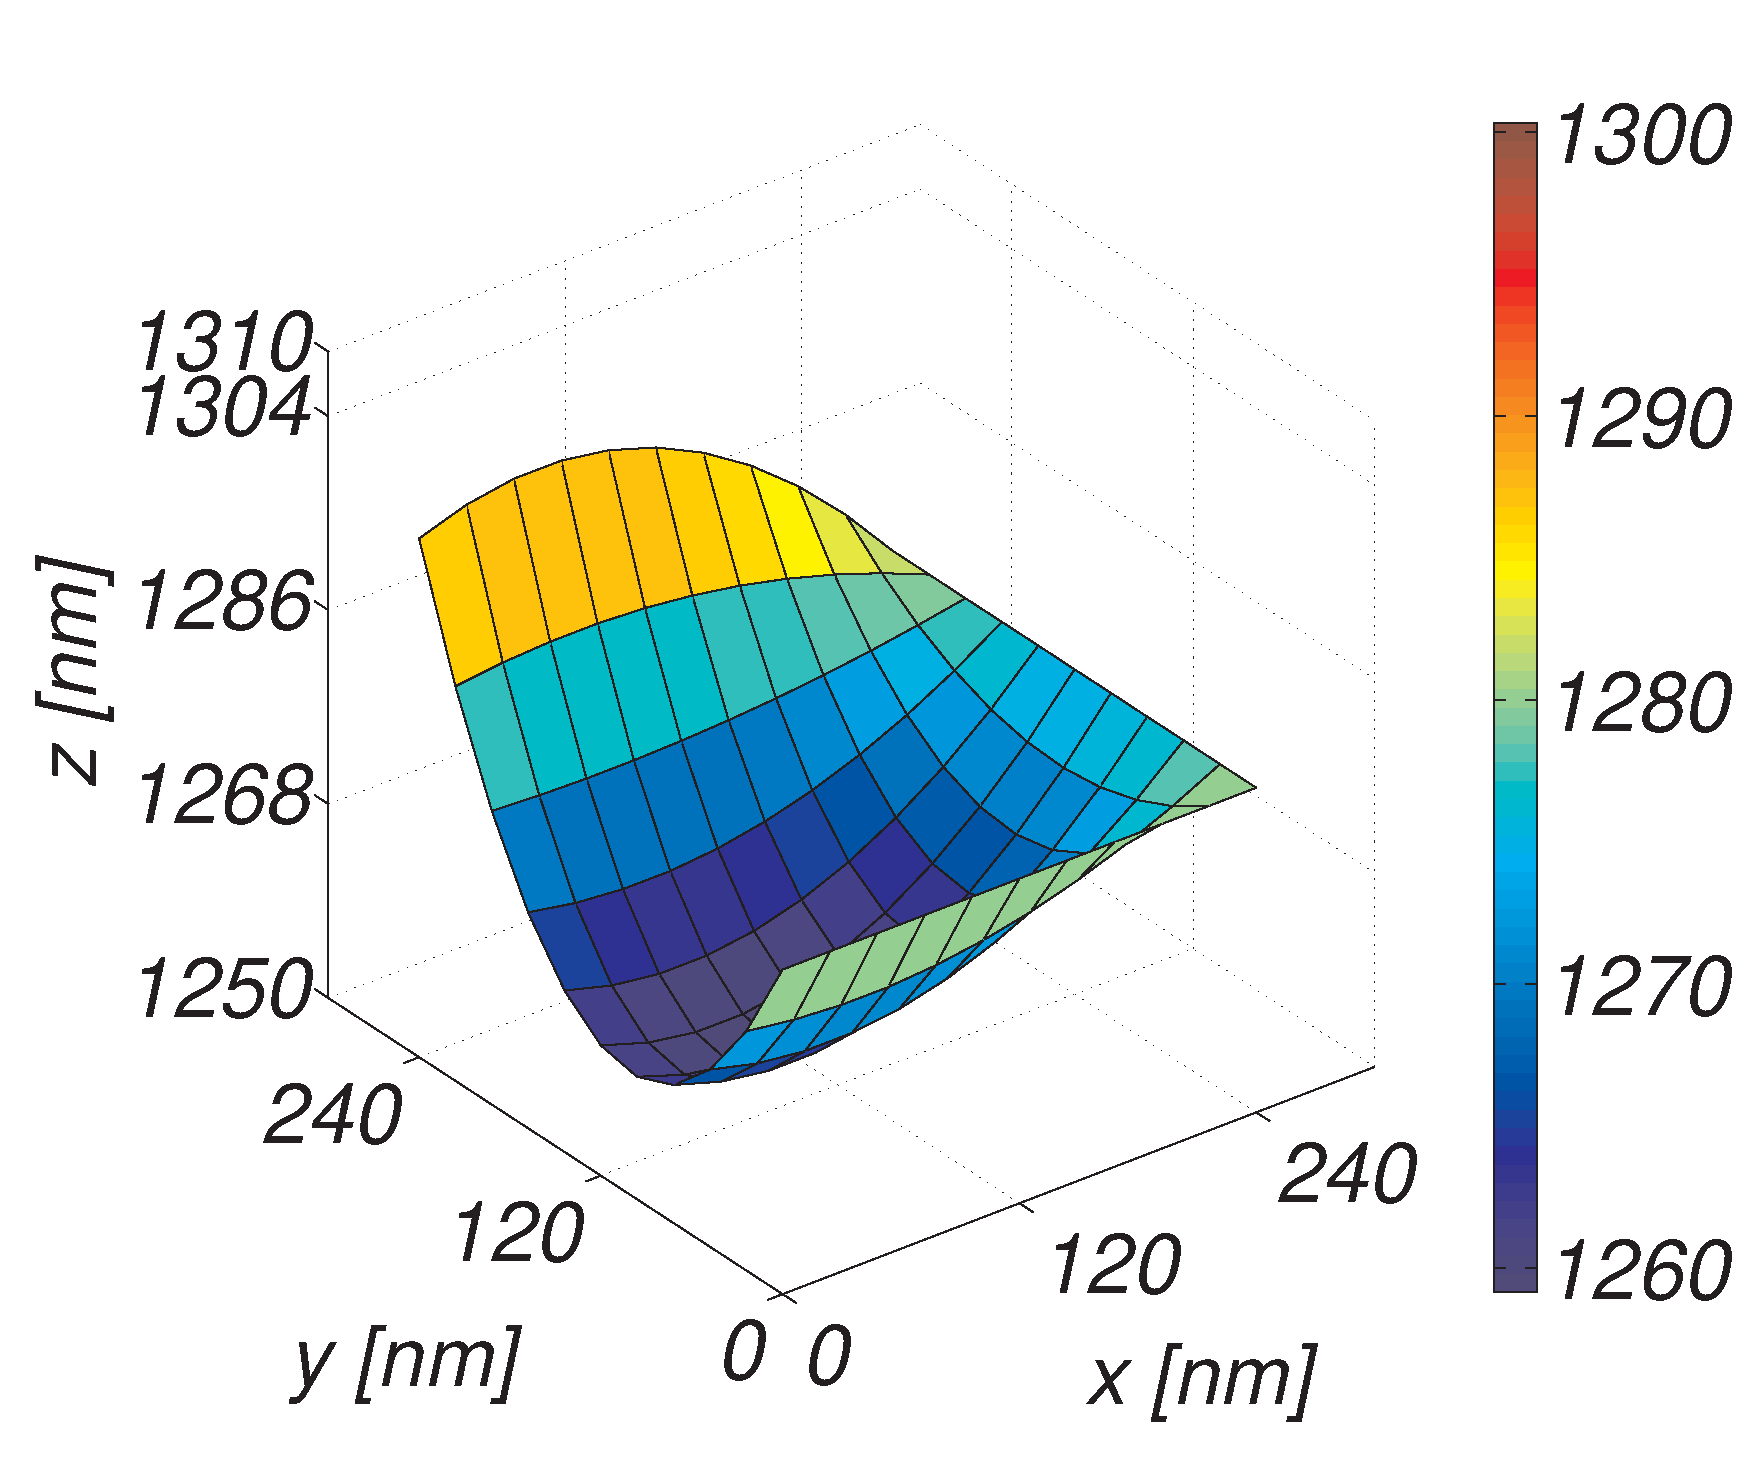
\includegraphics[width=0.8\columnwidth]{figures/eps/3x3_interpol2.eps}
		\caption{$3\times3$ mérési pont $11\times11$ pontba való interpolációja}
		\label{fig:33pont}
	\end{figure}
	
\subsection{Szimulálandó térfogat méretének számítása}
	A szimulálandó tér (hasáb) alapja adott az előzőleg említett interpolált felületként, míg a
	magassága nem. Ezt a következő két mennyiség közül a nagyobbikkal határoztuk meg:
	\begin{itemize}
		\item Középső pont fölött lévő tű közepének magassága,
		\item A ($3\times3$) környezet legalacsonyabb és legmagasabb pontjának
		különbsége.
	\end{itemize}
	A magasságtérkép egy vonalának részlete látható a \ref{fig:numh}. ábrán, 
	továbbá a szimulálandó tér (hasáb) magassága.
	
	\begin{figure}[!ht]
		\centering
		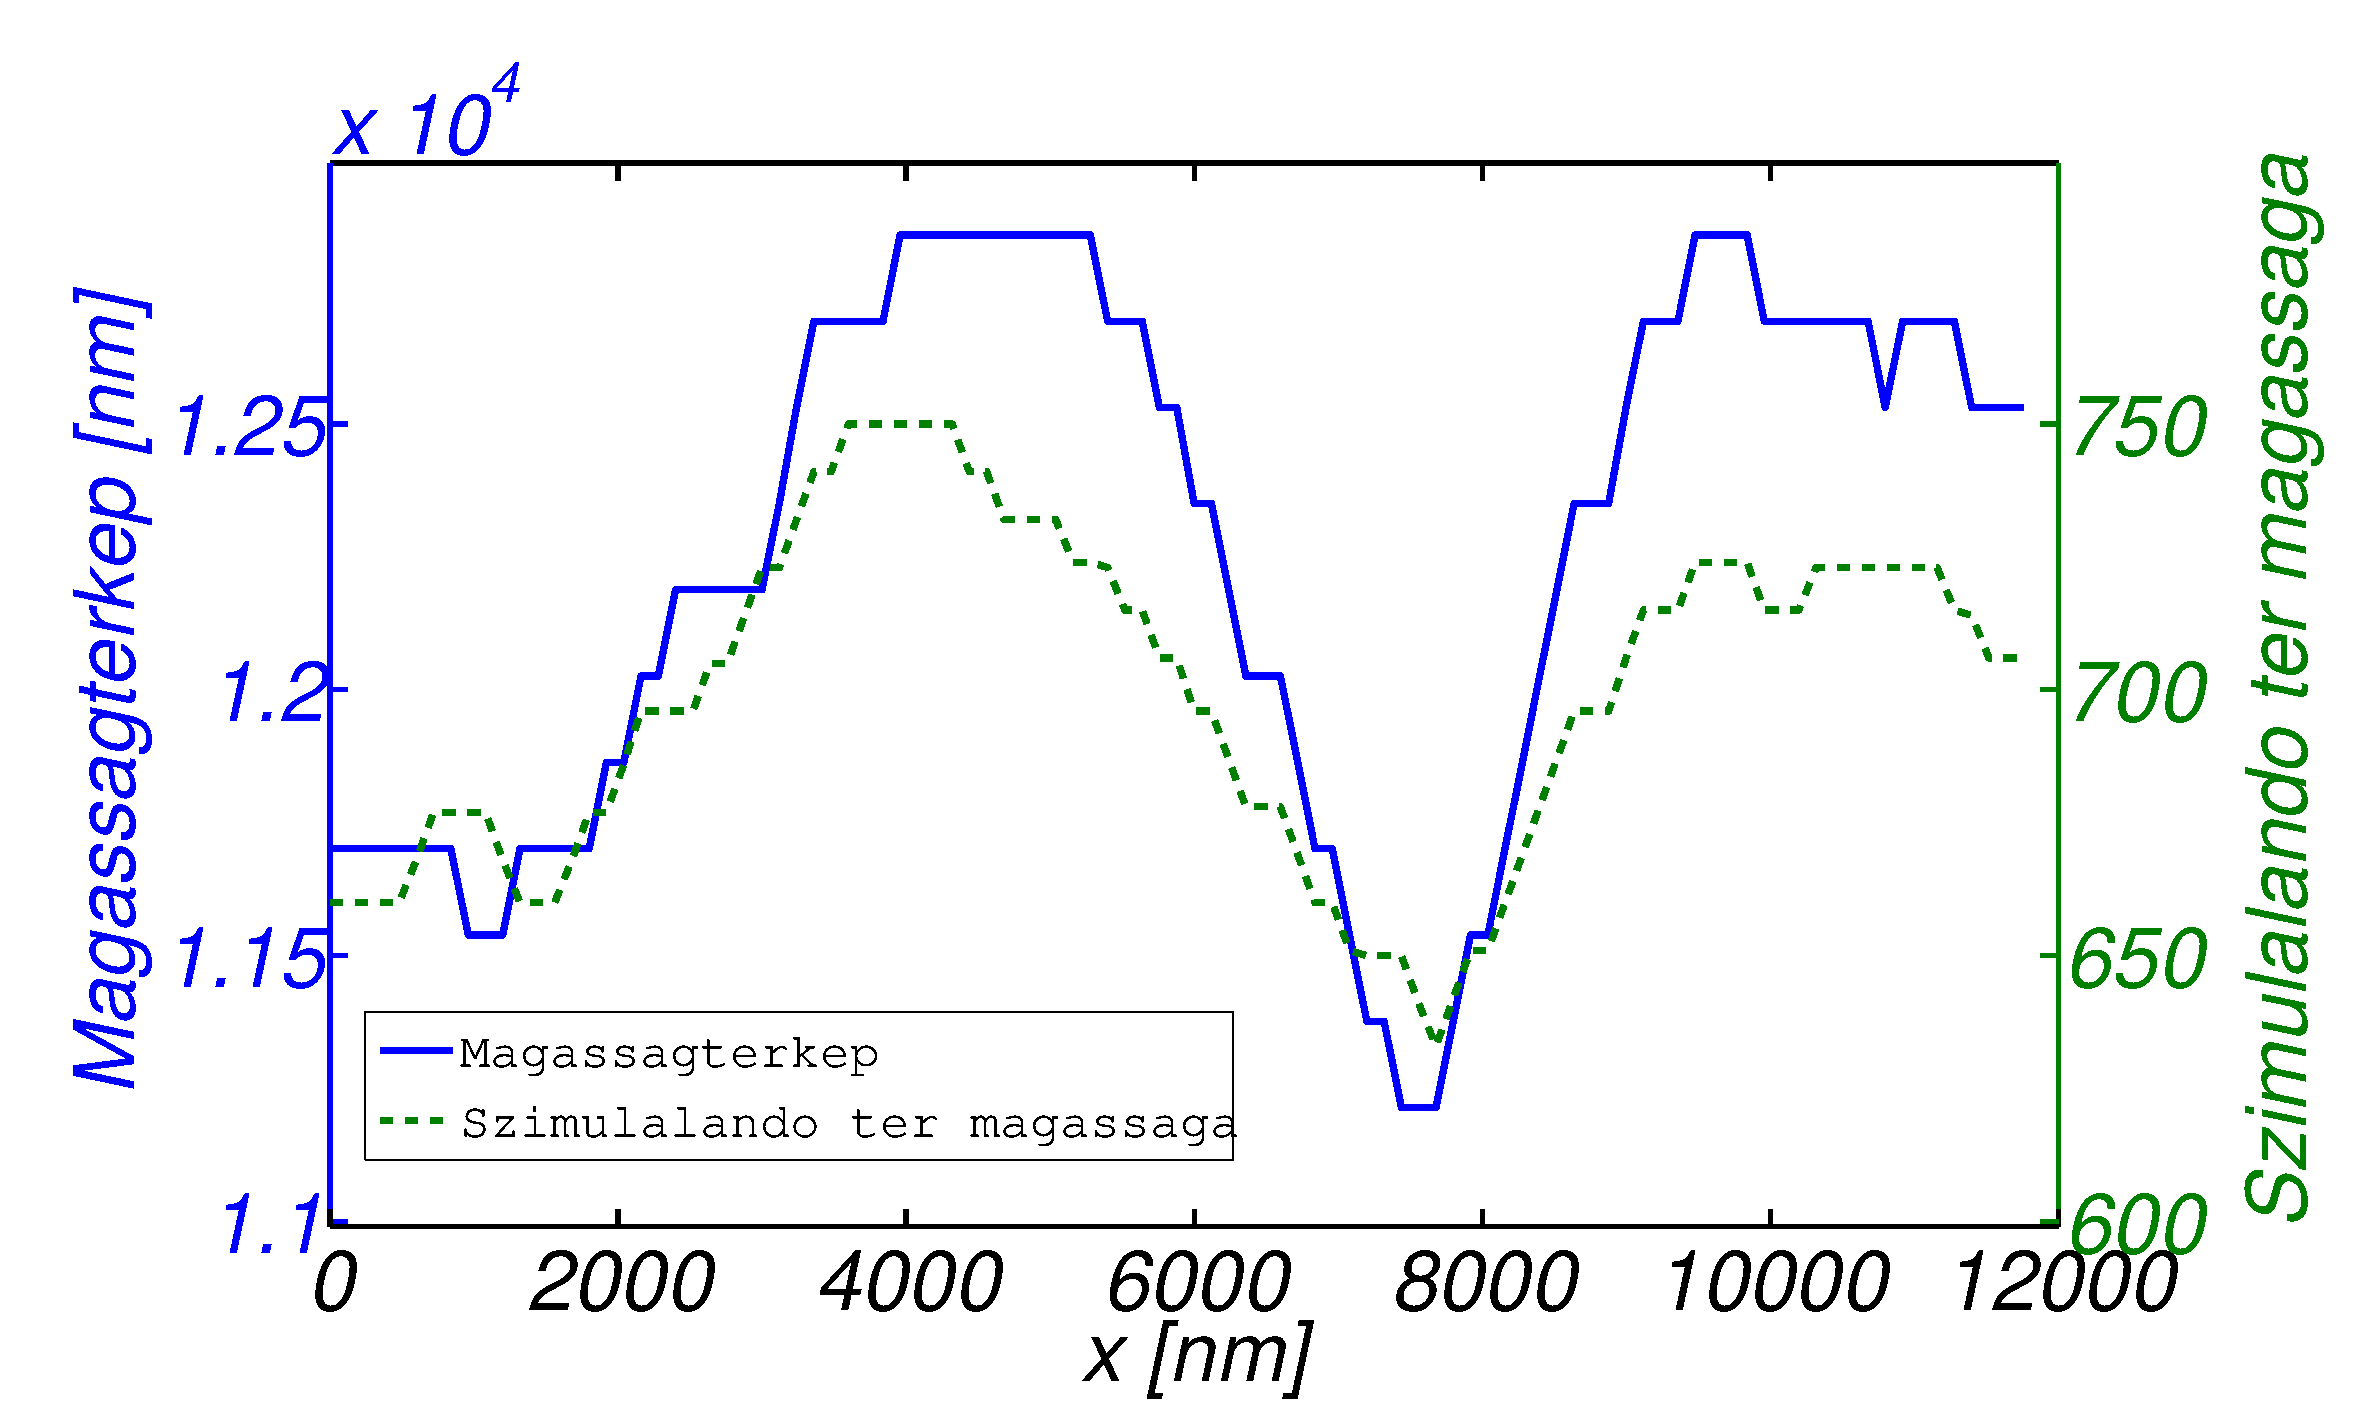
\includegraphics[width=0.7\columnwidth]{figures/eps/numh_vonal.eps}%
		\caption{A mérési eredmény egy vonal menti részlete (folytonos vonal) és az ezen
		mérési pontokhoz számított szimulációs tér magassága (szaggatott-vonal)}
		\label{fig:numh} 
	\end{figure}

	
\subsection{Iteratív megoldó algoritmus}
	Az iterációhoz a térháló pontjaihoz két mátrixot (tömbböt) rendelünk, ami a
	pontok potenciáljának aktuális ($\mathbf{V_{now}}$) és előző ($\mathbf{V_{prev}}$)
	értékeit tartalmazza.
	Az aktuális értékeket \eqref{eq:it} szerint számítjuk, majd az egész térre
	számítjuk az előzővel vett különbségének négyzetösszegét (normáját). E mérték
	képviseli a konvergencia szintjét, amit az iteráció során vizsgálva jutunk el a
	kívánt konvergencia szintre.
	Ha nem értük el a konvergencia szintet, akkor az előző két mátrixot
	felcserélve iterálunk tovább.
	
\subsection{Adatok mentése}
	Tesztelhetőségi megfontolások végett nem csak a tűre ható erőt (villamos
	térerősséget) exportáljuk, hanem a konvergencia szintjének változását és az
	interpolált felületet is. Az exportálandó menyiségek ``kis''
	mérete miatt egyszerű *.csv fájlként kerülnek mentésre. Ezen fájlok további
	poszt-processzálása MATLAB vagy munkalap kezelő szoftverrel is elvégezhető.

\section{Implementációhoz szükséges megfontolások}
	
	A következőkben egy kissebb teljesítményű notebook videókártyát veszek
	alapul a megfontolások demonstrálására. Ez az nVidia GeForce 330M, 
	575 MHz-en futó 48 CUDA core-al, 1024GB memóriával és
	OpenCL 1.0 kompatibilitással.
	A videókártya továbbiakban fontos paraméterei a \ref{table:vcard}. táblázatban
	látható.
	
	\begin{table}[!h]
	\renewcommand{\arraystretch}{1.3}
	% if using array.sty, it might be a good idea to tweak the value of
	% \extrarowheight as needed to properly center the text within the cells
	\caption{nVidia GeForce 330M OpenCL tulajdonságai}
	\label{table:vcard}
	\centering
	% Some packages, such as MDW tools, offer better commands for making tables
	% than the plain LaTeX2e tabular which is used here.
	\begin{tabular}{l|r}
		MAX\_COMPUTE\_UNITS & 6\\
		MAX\_WORK\_GROUP\_SIZES & 512 512 64\\
		GLOBAL\_MEM\_SIZE & 1073020928\\
		MAX\_CONSTANT\_BUFFER\_SIZE & 65536\\
		LOCAL\_MEM\_SIZE & 16384
	\end{tabular}
	\end{table}
	
	Ha a tér, ahol a laplace egyenletet meg kell oldanunk nagyon nagy, akkor
	érdemes szétbontani kissebb alterekre és azokhoz rendelni egy-egy
	``work-item''-et. Mivel a diszkrét Laplace egyenlet egy pontja a szomszédos
	pontokkal szoros kapcsolatban van, így az összefüggő ``work-item"-eket egy
	``work-group''-ba érdemes szervezni, mivel így az átlapolódó pontok értékét a
	szomszédos ``work-item''-ek is tudják írni és olvasni. Az ilyen típusú
	problémának méretét a MAX\_WORK\_GROUP\_SIZES tulajdonság korlátozza.
	
	Jelen esetben a mérési eredmény egy pontjához tartozó tér átlagosan
	$11\times11\times30$ pontból áll.
	Tehát a korábbi nem áll fenn és egyszerű megfeleltetéssel szétoszthatjuk a
	feladatot.
	A teljes tér $512\times512\times11\times11\times30$ méretű, ami $951k$ pont.
	A tárolásához single-precision mellett ennek a számnak a 4-szerese
	szükségeltetik byte-okban mérve. Mivel ez a videókártyán nem áll
	rendelkezésre, így szétbontjuk kissebb feladatrészekre.
	
	Ezen feladatrészek méretét egy paraméter állításával lehet változtati és az
	implementált algoritmus ettől generikusan függ.
	Emellett az interpoláció mértéke $N_{ip}$ is paraméterrel generikusan állítható.
	Az algoritmus generikusságát csupán a futási időben történő dinamikus memória
	allokációval lehetséges megvalósítani. A korábban említettek végett (\ref{table:mem} táblázat)
	az allokáció csak a ``host'' programban történhet.

\section{Memória szervezés}
\subsection{Csak globális memória használata}
	Az algoritmus pszeudó kódjának direkt leképezése esetén a ``host''-on
	allokálunk memóriát a ``device'' globális memóriájában,
	majd a megfelelő adatokat ide másoljuk és a kernel is itt ír és olvas.
	A problémát a globális memória nagy hozzáférési ideje jelenti, ami miatt sok
	``work-item'' tétlenül a memóriára fog várakozni.
	Ilyenkor az egy mérési pontra vonatkoztatott szimulációs idő a
	referenciánál is lassabb.
\subsection{Globális memória és adott esetben lokális memória használata}
	Kis erőfeszítéssel nagy javulást lehet elérni, ha a mérési ponthoz tartozó
	szimulációs tér éppen belefér a lokális memóriába.
	Tehát, mielőtt az \eqref{eq:it} szerinti iteratív megoldót futtatnánk először a
	globális memóriából a lokális memóriába töltjük át a kérdéses pontokat, majd
	számolunk rajta és a végén visszatöltjük a globális memóriába.
	E javítással a referenciával azonos sebességet tudunk elérni.
\subsection{Globális memória és minden adódó alkalomkor a lokális memória használata}
	Nagyobb erőfeszítést igényel, hogy minden alkalommal a globális memóriával való kommunikációt a
	lokális memória közbeékelésével tegyük.
	Ezt úgy lehet felfogni, mintha a globális memóriát lokális memória méretű
	kvantumokban tudnám csak elérni.
	Ekkor nagy odafigyelést kíván a memóriacímzés megfelelő prgramozása, de
	eredményképp gyorsulás érhető el. \\
	
	\noindent
	\begin{center}
	Összegezve elmondható, hogy az aktuálisan használt adat tárolását a lehető
	legközelebb kell tartani a ``compute-unit''-hoz.
	\end{center}
	
	\begin{table*}[!Ht]
		%\renewcommand{\arraystretch}{1.2}
		% if using array.sty, it might be a good idea to tweak the value of
		% \extrarowheight as needed to properly center the text within the cells
		\caption{OpenCL futási idő eredmények $12\times12$ mérési pontra}
		\label{table:openresult}
		% Some packages, such as MDW tools, offer better commands for making tables
		% than the plain LaTeX2e tabular which is used here.
		\centering
		\begin{tabular}{l|r|r|r}
		 & Globális memória & Lokális memória, ha befér & Lokális memória bufferelés\\ \hline
		\parbox{2.5cm}{Globális tranzakciók száma átlagosan} & $12 \times 12\times 32.3$
		& $12 \times 12 \times 32.3$ & $12 \times 12 \times 32.3$\\
		\parbox{2.5cm}{Lokális tranzakciók száma átlagosan} & 0 &
		$0.48 \times 12 \times 12 \times 30$ & $2.08 \times 12 \times12 \times 32.3$\\
		Futási idő & 5990 ms & 2530 ms & 510 ms\\
		Fajlagos futási idő & 410 ms & 170 ms & 3.5 ms 
		\end{tabular}
	\end{table*}
	